\documentclass[a4paper,12pt]{article}

\usepackage[utf8]{inputenc}
\usepackage[T1]{fontenc}
%\usepackage{graphicx}
%\usepackage[parfill]{parskip}
%\usepackage{url}
\usepackage{amssymb}
\usepackage{amsmath}
%\usepackage{caption}
%\usepackage{subcaption}
%\usepackage{tabularx}
%\usepackage{floatrow}
%\usepackage{multirow}
%\usepackage{cancel}
%\usepackage{siunitx}
%\usepackage{color}
%\usepackage{arydshln}
\usepackage{epigraph}				% funny quotes
%\usepackage{booktabs}
%\usepackage{fancyhdr}
%\usepackage{geometry}
%\usepackage{float}
%\usepackage[numbered]{mcode}
\usepackage{bm}						% vector/matrix typesetting
\usepackage[hidelinks]{hyperref}	% avoid red boxes on crossrefs
%\usepackage[round]{natbib}
%\usepackage[activate={true,nocompatibility},final,tracking=true,kerning=true,spacing=nonfrench,factor=1100,stretch=10,shrink=10]{microtype}

\newcommand{\M}[1]{\bm{#1}} 				% Use for variable matrices
\newcommand{\Mc}[1]{\mathbf{#1}} 			% Use for constant matrices (I, etc.)
\newcommand{\V}[1]{\mathbf{#1}} 			% Use for vectors
\newcommand{\transpose}{^{\text{T}}} 		% Make a guess, bitch
\newcommand{\sub}[1]{_{\textnormal{#1}}} 	% For upright subscript

% \lstset{
%     frame=single,
%     breaklines=true,
%     postbreak=\raisebox{0ex}[0ex][0ex]{\ensuremath{\color{green}\hookrightarrow\space}}
%     breaklines=true,
%     frame=topbottom
% }
% \hypersetup{
% 	colorlinks,
% 	citecolor=black,
% 	filecolor=black,
% 	linkcolor=black,
% 	urlcolor=black
% }
%\restylefloat{table}
%\captionsetup[table]{skip=10pt}
%\numberwithin{equation}{subsection}
%\allowdisplaybreaks
%\pagestyle{fancy}
%\fancyhf[HRE,HLO]{}
    
\begin{document}
\tableofcontents

\newpage
\epigraph{\textit{'Smack my pitch up.'}}{The Prodigy (1997)}

\section{Optimal control of pitch/travel without feedback}

%%%%%%%%%%%%%%%%%%%%%%%%%%%%%%%%%%%%%%%%%%%%%%%%%%%%%%%%%%%%
\subsection{State space form (10.2.1)}
%%%%%%%%%%%%%%%%%%%%%%%%%%%%%%%%%%%%%%%%%%%%%%%%%%%%%%%%%%%%
We want to write the model \eqref{eq:model1} in continuous time state space form with states and input as shown in \eqref{eq:state_and_input}.

\begin{equation}\label{eq:model1}
	\V{\dot{x}} = \M{A}_{c}\V{x} + \M{B}_{c}u
\end{equation}

\begin{subequations}\label{eq:state_and_input}
\begin{align}
	\V{x} 	&= \begin{bmatrix}\lambda & r & p & \dot{p} \end{bmatrix}\transpose \\
	u 		&= p_{c}
\end{align}
\end{subequations}

The equations of motion for the states are shown in \eqref{eq:state_equations} and the constants used are defined in \eqref{eq:K1K2}.

\begin{subequations}\label{eq:state_equations}
\begin{align}
	\dot{\lambda} 	&= r \\
	\dot{r} 		&= - K_{a} p \\
	\dot{p} 		&= \dot{p} \\
	\ddot{p} 		&= K_{1} K_{pp} (p_{c} - p) - K_{1} K_{pd} \dot{p}
\end{align}
\end{subequations}

\begin{subequations}\label{eq:K1K2}
\begin{align}
	K_{1} &= \frac{K_{f} l_{n}}{J_{p}} \\
	K_{2} &= \frac{K_{p} l_{a}}{J_{t}}
\end{align}
\end{subequations}

The above gives the result in \eqref{eq:state_space_matrices}.

\begin{equation}\label{eq:state_space_matrices}
	\V{\dot{x}} =
	\underbrace{
		\begin{bmatrix}
			0 & 1 & 0 				& 0 \\
			0 & 0 & -K_{2} 			& 0 \\
			0 & 0 & 0 				& 1 \\
			0 & 0 & -K_{1}K_{pp}	& -K_{1}K_{pd}
		\end{bmatrix}
	}_{\M{A}_{c}}
	\V{x} +
	\underbrace{
		\begin{bmatrix}
			0 \\ 0 \\ 0 \\ K_{1}K_{pp}
		\end{bmatrix}
	}_{\M{B}_{c}}
	u
\end{equation}


%%%%%%%%%%%%%%%%%%%%%%%%%%%%%%%%%%%%%%%%%%%%%%%%%%%%%%%%%%%%
\subsection{Model discussion (10.2.1)}
%%%%%%%%%%%%%%%%%%%%%%%%%%%%%%%%%%%%%%%%%%%%%%%%%%%%%%%%%%%%
The states are travel, travel rate, pitch, and pitch rate. The controller output is the pitch setpoint to be used by the already implemented controller which in turn calculates voltage inputs for the plant. Thus, we are modelling not the helicopter alone, but a system that consists of the helicopter along with the given controller. This corresponds with Figure 7 (proper ref here?) in the exercise text (add ref).


%%%%%%%%%%%%%%%%%%%%%%%%%%%%%%%%%%%%%%%%%%%%%%%%%%%%%%%%%%%%
\subsection{Discretisation (10.2.2)}
%%%%%%%%%%%%%%%%%%%%%%%%%%%%%%%%%%%%%%%%%%%%%%%%%%%%%%%%%%%%
We discretise the system by the Forward Euler Method. The general definition of the method and how it relates to our system is described by equations \eqref{eq:forward_euler} and \eqref{eq:euler_func}, respectively.

\begin{equation}\label{eq:forward_euler}
	y_{k+1} = y_{k} + h f(x_{k}, y_{k})
\end{equation}

\begin{equation}\label{eq:euler_func}
	f = \left( \M{A}_{c} \V{x}_{k} + \M{B}_c u_{k} \right)
\end{equation}

Using \eqref{eq:forward_euler} and \eqref{eq:euler_func}, we can find the matrices of the discretised system, as shown in \eqref{eq:disc} and \eqref{eq:disc_matrices}.

\begin{subequations}\label{eq:disc}
\begin{align}
	\V{x}_{k+1} &= \V{x}_{k} + \left( \M{A}_{c} \V{x}_{k} + \M{B}_c u_{k} \right) h \\
				&= \V{x}_{k} + h\M{A}_{c}\V{x}_{k} + h\M{B}_{c}u_{k} \\
				&= \left( \Mc{I} + h\M{A}_{c} \right) \V{x}_{k} + h\M{B}_{c}u_{k} \\
				&= \M{A}\V{x}_{k} + \M{B}u_{k}
\end{align}
\end{subequations}

\begin{subequations}\label{eq:disc_matrices}
\begin{equation}
	\M{A} = \Mc{I} + h\M{A}_{c} =
	\begin{bmatrix}
		1 & h & 0 & 0 \\
		0 & 1 & -K_{2}h & 0 \\
		0 & 0 & 1 & h \\
		0 & 0 & -K_{1}K_{pp}h	& 1-K_{1}K_{pd}h
	\end{bmatrix}
\end{equation}
\begin{equation}
	\M{B} = h\M{B}_c =
	\begin{bmatrix} 0 \\ 0 \\ 0 \\ K_{1}K_{pp}h \end{bmatrix}
\end{equation}
\end{subequations}

%%%%%%%%%%%%%%%%%%%%%%%%%%%%%%%%%%%%%%%%%%%%%%%%%%%%%%%%%%%%
\subsection{Cost function discussion}
%%%%%%%%%%%%%%%%%%%%%%%%%%%%%%%%%%%%%%%%%%%%%%%%%%%%%%%%%%%%
- cost function has a focus on the error between $\lambda_i$ and $\lambda_f$
- is a quadratic function, least-square 

%%%%%%%%%%%%%%%%%%%%%%%%%%%%%%%%%%%%%%%%%%%%%%%%%%%%%%%%%%%%
\subsection{unwatend effect dicsussion}
%%%%%%%%%%%%%%%%%%%%%%%%%%%%%%%%%%%%%%%%%%%%%%%%%%%%%%%%%%%%
- when $\lambda = \lambda_f$, you will minimize the pitch, making it 0. This can make the helicopter oscilate around $\lambda = \lambda_f$, as the pitch will be set to 0 on that particular point

%%%%%%%%%%%%%%%%%%%%%%%%%%%%%%%%%%%%%%%%%%%%%%%%%%%%%%%%%%%%
\subsubsection{4 does the helicopter end in desired and what causes deviation}
%%%%%%%%%%%%%%%%%%%%%%%%%%%%%%%%%%%%%%%%%%%%%%%%%%%%%%%%%%%%
- No, because the optimization calculation doesn't take in account the brake time to stop in the desired point, and thus it doesn't stop in time.


\newpage
\epigraph{\textit{'I've got 99 problems, but a pitch ain't one.'}}{Ice-T (1993)}
\section{Optimal control of pitch/travel with LQ control}

\section{MPC discussion}

\subsubsection{how would you realize MPC}
look at exercise 

\subsubsection{discuss advantages and disadvantages with MPC compared to the one you have implemented}
MPC: a lot of computations, heavy for the computer, slow, but very accurate
LQR: not that much computations, generally fast, not that accurate

\subsubsection{think about how the structure in fig 8 would look if you used MPC}

\newpage
\section{Optimal control of pitch/travel and elevation with and without feedback}

\newpage
\section{Pastebin (remove before handing in lol)}

%%%%%%%%%%%%%%%%%%%%%%%%%%%%%%%%%%%%%%%%%%%%%%%%%%%%%%%%%%%%
\subsection{Bibtex test}
%%%%%%%%%%%%%%%%%%%%%%%%%%%%%%%%%%%%%%%%%%%%%%%%%%%%%%%%%%%%
\cite{nocedal_numerical_2006} and \cite{_helicopter_2015} are pretty cool.

%%%%%%%%%%%%%%%%%%%%%%%%%%%%%%%%%%%%%%%%%%%%%%%%%%%%%%%%%%%%
\subsection{mcode test}
%%%%%%%%%%%%%%%%%%%%%%%%%%%%%%%%%%%%%%%%%%%%%%%%%%%%%%%%%%%%
\lstinputlisting[label={lst:dog}, caption={A dog.}]{blkdiag.m}

\begin{figure}[H]
	\centering
	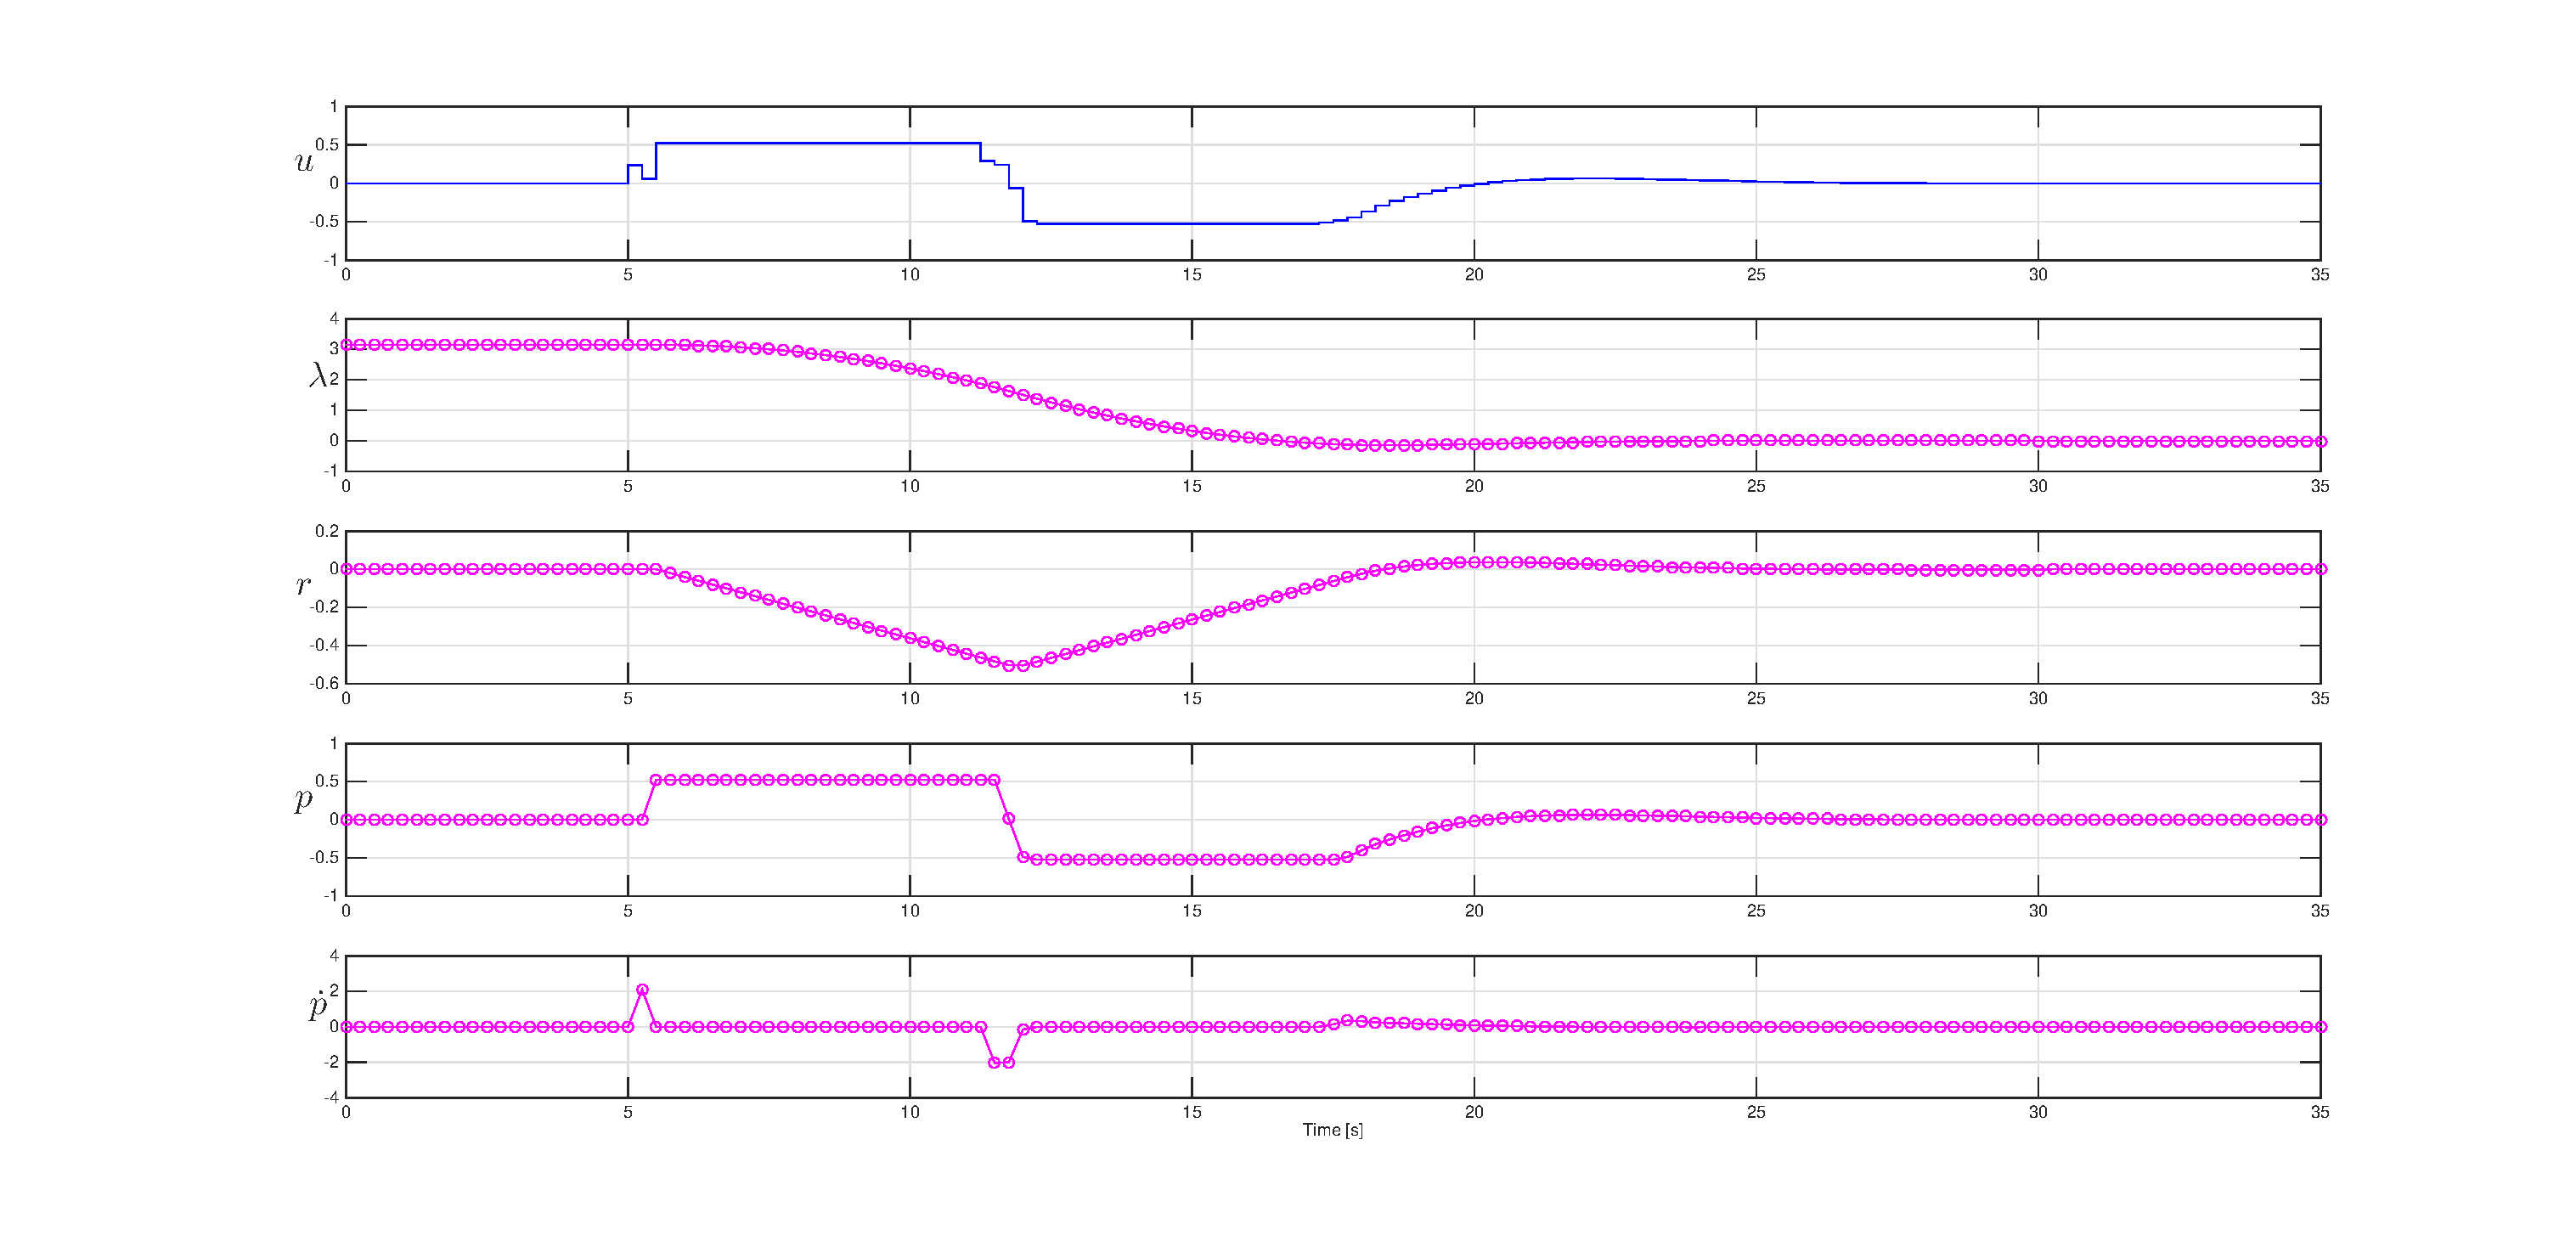
\includegraphics[width=\textwidth]{Opp10_3-good}
	\caption{Digraph.}
	\label{fig:digraph}
\end{figure}


\end{document}
